\documentclass[italian,10pt,a4paper]{article}
\usepackage[T1]{fontenc}
\usepackage{graphicx}
\usepackage{mathtools}
\usepackage{amssymb}
\usepackage{amsthm}
\usepackage{thmtools}
\usepackage{xcolor}
\usepackage{nameref}
\usepackage{longtable}
\usepackage{tabularray}
\usepackage{tabularx}
\usepackage{microtype}
\usepackage{cancel}
\usepackage{babel}
\usepackage[hidelinks]{hyperref}
\usepackage{mdframed}
{\renewcommand{\arraystretch}{2}%
\title{Appunti di parallel programming}
\author{Riccardo Torre\and Michele Perlotto}
\newtheoremstyle{note}% <name>
{3pt}% <Space above>
{3pt}% <Space below>
{}% <Body font>
{}% <Indent amount>
{\bfseries}% <Theorem head font>
{:}% <Punctuation after theorem head>
{.5em}% <Space after theorem headi>
{}% <Theorem head spec (can be left empty, meaning `normal')>
\theoremstyle{note}
\newtheorem{exercise}{Esercizio}[section]
\newtheorem{solution}{Soluzione}[section]
%\theoremstyle{definition}
\begin{document}
	\maketitle
	\tableofcontents
	\section{Introduzione}
Un programma eseguito su un'architettura dotata di una singola unità di elaborazione centrale (CPU) può essere eseguita esclusivamente in maniera sequenziale (un'istruzione alla volta) in figura \ref{fig:single-computation}.
% TODO: \usepackage{graphicx} required
\begin{figure}[th]
	\centering
	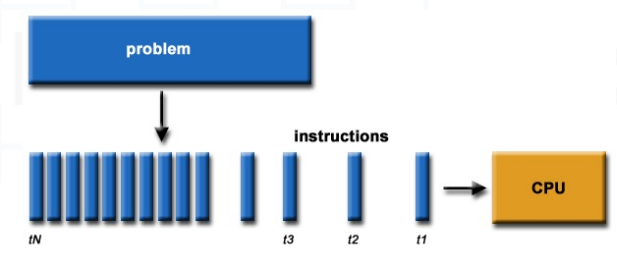
\includegraphics[width=0.7\linewidth]{img/single-computation}
	\caption{esecuzione su un'architettura dotata di una sola CPU.}
	\label{fig:single-computation}
\end{figure}
Nel senso più semplice, il \textbf{calcolo parallelo} è l'uso simultaneo di più risorse di calcolo per risolvere un problema computazionale. A differenza della soluzione sequenziale, l'esecuzione avviene su più di una CPU e il problema iniziale (il programma) viene suddiviso in sottoproblemi che a loro volta vengono suddivisi in una serie di istruzioni. L'esecuzione del programma avviene in maniera simultanea (figura \ref{fig:parallel-computation}).
\begin{figure}[th]
	\centering
	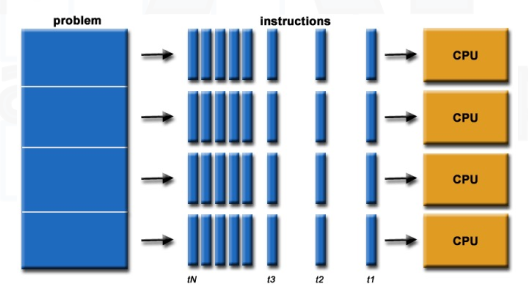
\includegraphics[width=0.7\linewidth]{img/parallel-computation}
	\caption{esecuzione parallela su un'architettura che supporta più di una CPU.}
	\label{fig:parallel-computation}
\end{figure}

	\section{Terminologia e concetti}
L'architettura di Von Neumann è composta da quattro componenti principali:
\begin{enumerate}
	\item memoria;
	\item unità di controllo (CU): recupera istruzioni/dati dalla memoria, decodifica le istruzioni e poi in \textbf{sequenza} coordina le operazioni per portare a termine il compito programmato;
	\item unità logico aritmetica (ALU): esegue operazioni aritmetiche di base;
	\item sistemi di I/O (input/output): interfaccia uomo-macchina.
\end{enumerate}
La \textbf{tassonomia classica di Flynn} distingue le architetture di computer multiprocessore in base a come possono essere classificate in due dimensioni indipendenti di \textbf{istruzioni} e \textbf{dati}.
Nella tassonomia di Flynn, vengono identificate cinque componenti:
\begin{enumerate}
	\item IS (Instruction Stream): ovvero il flusso di istruzioni del programma che deve essere eseguito;
	\item DS (Data Stream): il flusso degli operandi e dei risultati dei programmi che sono in esecuzione;
	\item CU (Control Unit): elemento funzionale (chi esegue il fetch e il decode, ovvero il recupero e la decodifica dei dati/istruzioni);
	\item PU (Processing Unit): unità funzionale composta dalla ALU e dai registri. Esegue le istruzioni;
	\item MM(Main Memory): la memoria dove i dati e le istruzioni sono allocati.
\end{enumerate}
Le possibili classificazioni sono:
\begin{enumerate}
	\item SISD (Single Instruction Single Data): la CU recupera le istruzioni dalla MM, mentre la PU esegue le istruzioni interagendo con MM per modificare i dati (figura \ref{fig:sisd});
	\begin{figure}[th]
		\centering
		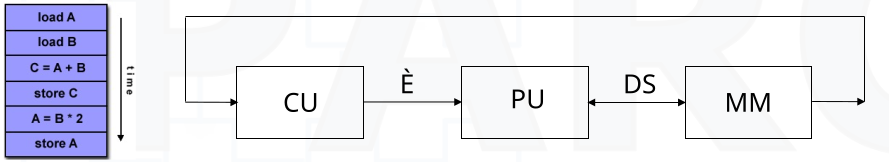
\includegraphics[width=0.7\linewidth]{img/sisd}
		\caption{Single Istruction Single Data.}
		\label{fig:sisd}
	\end{figure}
	\item SIMD (Single Instruction Multiple Data): tutte le unità di elaborazione eseguono la stessa istruzione in ogni dato ciclo di clock; ogni unità di elaborazione può operare su un dato diverso (figura \ref{fig:simd}); è ideale per problemi specializzati caratterizzati da un elevato grado di regolarità, come l'elaborazione grafica o l'elaborazione di immagini; esecuzione sincrona (\textbf{lockstep}) e deterministica
	\begin{figure}[th]
		\centering
		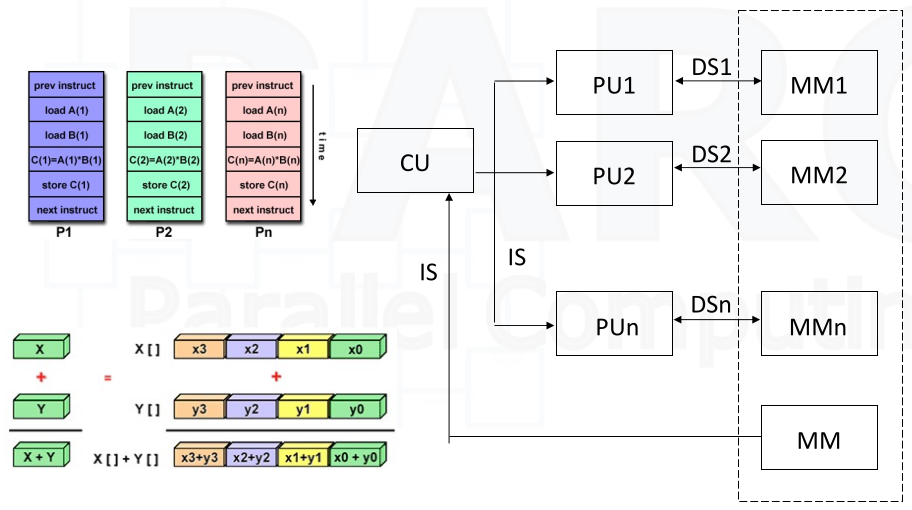
\includegraphics[width=0.7\linewidth]{img/simd}
		\caption{Single Istruction Multiple Data.}
		\label{fig:simd}
	\end{figure}

	\item MISD (Multple Instruction Single Data): un singolo flusso di dati viene immesso in più unità di elaborazione che opera sui dati in modo indipendente tramite flussi di istruzioni indipendenti. Sono esistiti pochi esempi reali di questa classe di computer paralleli (figura \ref{fig:misd});
	\begin{figure}[th]
		\centering
		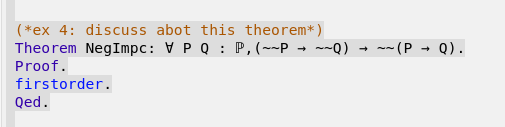
\includegraphics[width=0.7\linewidth]{img/misd}
		\caption{Multiple Instruction Single Data.}
		\label{fig:misd}
	\end{figure}

	\item MIMD (Multple Instruction Multple Data): è il tipo più comune di computer parallelo; ogni processore può eseguire un flusso di istruzioni diverso e lavorare con un flusso di dati diverso. L'esecuzione può essere sincrona o asincrona, deterministica o non deterministica (figura \ref{fig:mimd}).
	\begin{figure}[!th]
		\centering
		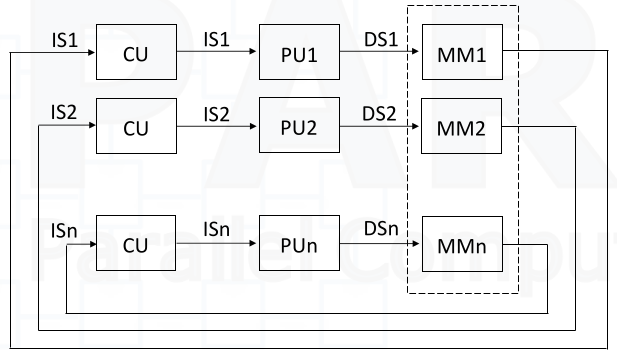
\includegraphics[width=0.7\linewidth]{img/mimd}
		\caption{Multiple Instruction Multiple Data.}
		\label{fig:mimd}
	\end{figure}

\end{enumerate}
\subsection{Terminologia delle architetture parallele}

	\begin{longtable}{|m{0.28\linewidth}|m{0.62\linewidth}|}
		\hline
		\textbf{Termine} & \textbf{Significato}
		\\
		\hline
		\textbf{Task (sequenziale)} & È un'unità di esecuzione o di lavoro di un programma o di un sottoprogramma. Le istruzioni sono eseguite sequenzialmente ovvero non in parallelo.
		\\
		\hline
		\textbf{Task parallelo}& È un task che può essere eseguito in modo sicuro su più processori. Ciascuna istruzione di un task può essere eseguita in maniera concorrente.
		\\
		\hline
		\textbf{Esecuzione seriale} & È l'esecuzione di un programma in sequenza, una dichiarazione alla volta. Nel senso più semplice questo accade su una macchina con un processore. Tuttavia, praticamente tutte le attività parallele avranno sezioni di un programma parallelo che devono essere eseguite in serie.
		\\
		\hline
		\textbf{Esecuzione parallela} & È l'esecuzione di un programma da più di un task, in cui ogni attività è in grado di eseguire la stessa o una diversa istruzione simultaneamente.
		\\
		\hline
		\textbf{Pipelining} & Suddivisione di un compito in passaggi eseguiti da diverse unità di elaborazione, con input che scorrono proprio come una catena di montaggio; un tipo di calcolo parallelo.  La pipeline è un tipo di architettura hardware utilizzata nel progetto dei microprocessori per incrementarne la produttività, ovvero la quantità di istruzioni eseguite nell'unità di tempo. Le istruzioni possono essere di un programma sequenziale. La pipeline può riferirsi anche ad una pipeline di task (ottimizzazione per GPU).
		\\
		\hline
		\textbf{Memoria condivisa} & Dal punto di vista strettamente hardware, descrive un'architettura informatica alla quale tutti i processori hanno accesso diretto (solitamente basato su bus) alla memoria fisica comune; dal punto di vista software, descrive un modello in cui le attività parallele hanno tutte la stessa "immagine" di memoria (\textbf{spazio di indirizzamento comune}) e possono indirizzarsi e accedervi direttamente alle stesse locazioni di memoria logiche indipendentemente da dove esiste effettivamente la memoria fisica. Se lo spazio di indirizzamento non fosse condiviso, si parla di \textbf{memoria distribuita} (che è il contrario della memoria condivisa).
		\\
		\hline
		\textbf{Multiprocessore simmetrico (SMP)} & Architettura hardware in cui più processori condividono un unico spazio di indirizzi e accedono a tutte le risorse; la computazione avviene su memoria condivisa.
		\\
		\hline
		\textbf{Memoria distribuita} & Dal punto di vista hardware, si riferisce all'accesso alla memoria basato sulla rete per la memoria fisica che non è in comune. Il termine può fare riferimento anche ad un'implementazione software dove le attività possono vedere solo la memoria della macchina locale su una vista logica e devono utilizzare comunicazioni per accedere alla memoria su altre macchine su cui sono in esecuzione altre attività.
		\\
		\hline
		\textbf{Comunicazione} & Le attività parallele in genere necessitano di scambiare dati. Esistono tuttavia diversi modi per ottenere questo risultato, ad esempio tramite un bus di memoria condiviso o tramite una rete, tuttavia l'evento effettivo dello scambio di dati viene comunemente definita \emph{comunicazione} indipendentemente dal metodo utilizzato.
		\\
		\hline
		\textbf{Sincronizzazione} & È il coordinamento di attività parallele in tempo reale, molto spesso associato a comunicazioni. Spesso implementate da stabilire un punto di sincronizzazione all'interno di un'applicazione in cui un'attività non può procedere oltre finché un'altra attività non raggiunge lo stesso punto o logicamente equivalente. La sincronizzazione di solito comporta l'attesa di almeno un'altra attività e può quindi causare un aumento del tempo di esecuzione del clock delle applicazioni parallele.
		\\
		\hline
		\textbf{Granularità} & Nel calcolo parallelo, la granularità è una misura quantitativa del rapporto tra il calcolo e la comunicazione. La granularità può essere:
		\begin{itemize}
			\item \textbf{grossolana:} tra gli eventi di comunicazione vengono eseguite quantità di lavoro computazionale relativamente grandi;
			\item \textbf{fine:} tra gli eventi di comunicazione vengono eseguite quantità di lavoro computazionale relativamente piccole.
		\end{itemize}
		\\
		\hline
		\textbf{Accelerazione osservata} & È definita come: $speedup = \frac{execTimeSerial}{execTimeParallel}$ e rappresenta uno degli indicatori più semplici e utilizzati per la performance di un programma parallelo.
		\\
		\hline
		\textbf{Overhead parallelo} & È l'ammontare di tempo richiesto per coordinare task paralleli anziché per eseguire la parte utile del lavoro. L'overhead parallelo può includere fattori come:
		\begin{itemize}
			\item tempo di avvio dei task;
			\item tempo per le sincronizzazioni tra task;
			\item tempo per le comunicazioni di dati tra task;
			\item overhead del software imposto da compilatori paralleli, librerie, strumenti, sistema operativo, \dots
			\item tempo di completamento dei task.
		\end{itemize}
		\\
		\hline
		\textbf{Massivamente parallelo} &  Si riferisce all'hardware che comprende un dato sistema parallelo, dotato di molti processori. Il significato di "molti" continua ad aumentare, ma attualmente i computer più grandi possono essere costituiti da processori che si contano nell'ordine di centinaia di migliaia.
		\\
		\hline
		\textbf{Imbarazzantemente parallelo} & Indica l'azione di risolvere simultaneamente task simili ma indipendenti; la coordinazione tra task è quasi assente o completamente assente.
		\\
		\hline
		\textbf{Scalabilità} & Si riferisce alla capacità di un sistema parallelo (HW e/o SW) di dimostrare un aumento proporzionale della velocità parallela con l'aggiunta di più processori. I fattori che contribuiscono alla scalabilità includono:
		\begin{itemize}
			\item HW: in particolare larghezze di banda della memoria-cpu e comunicazioni attraverso la rete;
			\item l'algoritmo dell'applicazione;
			\item relativo all'overhead parallelo;
			\item caratteristiche specifiche dell'applicazione e codifica
		\end{itemize}
		\\
		\hline
		\textbf{Processori multi-core} & Processori in cui sono presenti più core su un singolo chip
		\\
		\hline
		\textbf{Computazione in cluster} & Utilizzo di una combinazione di unità di calcolo di base (processori, reti o SMP) per costruire un sistema parallelo.
		\\
		\hline
		\textbf{Supercomputing / Calcolo ad alte prestazioni} & Utilizzo delle macchine più veloci e più grandi al mondo per risolvere problemi molto complessi (le unità di calcolo di cui sono composti non devono necessariamente essere omogenei).
		\\
		\hline
		\textbf{Edge computing} & Distribuire il paradigma informatico che avvicina il calcolo e l'archiviazione dei dati al luogo in cui si trovano. Necessario per migliorare i tempi di risposta e risparmiare larghezza di banda.
		\\
		\hline
	\end{longtable}
\subsubsection{Tipi di memoria}
La \textbf{cache} è un'area di memoria estremamente veloce ma solitamente di un basso ordine di grandezza di capacità. Il suo scopo è di velocizzare l'esecuzione dei programmi.

La figura \ref{fig:uma} è un esempio di memoria condivisa. I computer paralleli con memoria condivisa variano ampiamente, ma generalmente hanno in comune la capacità di tutti i processori di accedere a tutta la memoria come spazio di indirizzi globale. Più processori possono funzionare in modo indipendente ma condividono le stesse risorse di memoria. Le modifiche in una posizione di memoria effettuate da un processore sono visibili a tutti gli altri processori. Le macchine a memoria condivisa possono essere divise in due classi principali in base ai tempi di accesso alla memoria:
\begin{enumerate}
	\item UMA (Unified Memory Access): i processori sono identici, il tempo e la modalità di accesso alla memoria sono gli stessi per tutti i processori (figura \ref{fig:uma}). A volte chiamato \textbf{CC-UMA} (\emph{Cache Coherent UMA}). \textbf{Coerenza} della cache significa che se un processore aggiorna una posizione nella memoria condivisa, tutti gli altri processori vengono a conoscenza dell'aggiornamento. La coerenza della cache viene raggiunta a livello hardware.
	\begin{figure}[th]
		\centering
		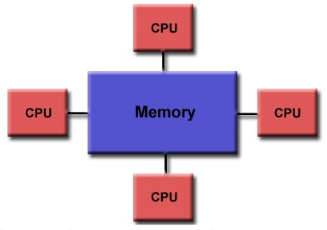
\includegraphics[width=0.7\linewidth]{img/UMA}
		\caption{Memoria condivisa di classe UMA.}
		\label{fig:uma}
	\end{figure}
	\item NUMA (Not Unified Memory Access): spesso realizzato collegando fisicamente due o più SMP; un SMP può accedere direttamente alla memoria di un altro SMP. Non tutti i processori hanno lo stesso tempo di accesso a tutte le memorie. L'accesso alla memoria attraverso il bus è più lento. Se viene mantenuta la coerenza della cache, la memoria si dice \textbf{CC-NUMA} (\emph{Cache Coherent NUMA}).
	\begin{figure}[th]
		\centering
		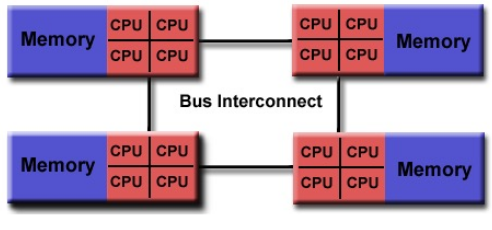
\includegraphics[width=0.7\linewidth]{img/NUMA}
		\caption{Memoria condivisa di classe NUMA.}
		\label{fig:numa}
	\end{figure}
\end{enumerate}
	\subsubsection{Vantaggi e svantaggi di una memoria condivisa.} Vantaggi di avere una memoria condivisa sono:
	\begin{itemize}
		\item lo spazio degli indirizzi globale fornisce alla memoria una prospettiva di programmazione user-friendly; \item la condivisione dei dati tra le attività è veloce e uniforme alla vicinanza della memoria alle CPU.
	\end{itemize}
	Gli svantaggi sono:
	\begin{itemize}
		\item mancanza di scalabilità tra memoria e CPU; \item diventa sempre più difficile e costoso progettare e produrre macchine a memoria condivisa con un numero sempre crescente di processori.
	\end{itemize}

Come i sistemi di memoria condivisa, i sistemi di memoria distribuita variano ampiamente ma condividono una caratteristica comune. Per connettere la memoria inter-processore, il sistema richiede una rete di comunicazione.
I processori hanno la propria memoria locale. Gli indirizzi di memoria in un processore non vengono mappati su un altro processore, quindi non esiste il concetto di \textbf{spazio degli indirizi globale} su tutti i processori.

Poiché ogni processore ha la propria memoria locale, funziona in modo indipendente. Le modifiche apportate alla memoria non hanno effetto sulla memoria degli altri processori. Pertanto, il concetto di coerenza della cache non si applica.
Quando un processore ha bisogno di accedere ai dati in un altro processore, solitamente è compito del programmatore definire esplicitamente come e quando i dati vengono comunicati. Anche la sincronizzazione tra i compiti è responsabilità del programmatore.

\subsubsection{Vantaggi e svantaggi di una memoria distribuita.} I vantaggi di avere una memoria distribuita sono:
\begin{itemize}
	\item la \textbf{memoria} è \textbf{scalabile} con il numero di processori; \item aumenta il numero di processori e la dimensione della memoria aumenta proporzionalmente; \item ogni processore può accedere rapidamente alla propria memoria senza interferenze e senza il sovraccarico sostenuto nel tentativo di mantenere la coerenza della cache. \item in termini di costi, la memoria distribuita è efficace, poiché può utilizzare processori e reti standard disponibili in commercio.
\end{itemize}
Gli svantaggi sono i seguenti:
\begin{itemize}
	\item il programmatore è responsabile per molti dei dettagli associati alla comunicazione dei dati tra i processori. \item potrebbe essere difficile mappare su questa organizzazione della memoria le strutture dati esistenti, basate sulla memoria globale; \item tempi di accesso alla memoria non uniforme (NUMA).
\end{itemize}
\subsubsection{Memoria ibrida distribuita-condivisa} I computer più grandi e veloci del  mondo oggi impiegano questo tipo di architettura (figura \ref{fig:hybrid-memory}). Il componente di memoria condivisa è solitamente una macchina SMP coerente con la cache. I processori su un dato SMP possono indirizzare la memoria di quella macchina come globale.

\begin{figure}[th]
	\centering
	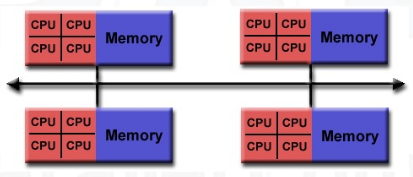
\includegraphics[width=0.7\linewidth]{img/hybrid-memory}
	\caption{Memoria ibrida distribuita-condivisa.}
	\label{fig:hybrid-memory}
\end{figure}

Il componente di memoria distribuita è il collegamento in rete di più SMP. Gli SMP conoscono solo la propria memoria, non quella di un altro SMP. Pertanto, le comunicazioni di rete sono necessarie per spostare i dati da un SMP all'altro. I vantaggi e gli svantaggi sono tutto ciò che è comune alle architetture di memoria e distribuita.

	\section{Modelli di programmazione parallela}
Esistono diversi modelli di programmazione parallela comunemente usati come la \textbf{memoria condivisa}, le \textbf{threads}, il \textbf{passaggio di messaggi}, il \textbf{parallelismo dei dati} e un approccio \textbf{ibrido}. Questi modelli sono un astrazione dell'hardware e delle architetture di memoria sottostanti.

Questi modelli non sono specifici di una particolare macchina o architettura di memoria. In effetti, ciascuno di questi modelli può essere implementato su qualsiasi hardware sottostante. Due esempi:
\begin{enumerate}
	\item modello di memoria condivisa su una memoria distribuita: approccio KSR (\textit{Kendall Square Research}) ALLCACHE. La memoria della macchina era distribuita fisicamente, ma appariva all'utente come un'unica memoria condivisa (spazio di indirizzi globale). Genericamente questo approccio viene definito come \textit{"macchina virtuale condivisa"};
	\item modello di passaggio del messaggio su una macchina con memoria condivisa. MPI su SGI Origin. SGI Origin utilizzava un'architettura di memoria condivisa di tipo CC-NUMA, in cui ogni attività ha accesso diretto alla memoria globale. Tuttavia, la capacità di inviare e ricevere messaggi con MPI, come avviene comunemente su una rete di macchine a memoria distribuita, non solo è implementata ma è utilizzata molto comunemente.
\end{enumerate}

Quale modello utilizzare è spesso una combinazione di ciò che è disponibile e di una scelta personale. Non esiste un modello "migliore", anche se esistono certamente implementazioni migliori di alcuni modelli rispetto ad altri.

\subsection{Modello di memoria condivisa} Nel modello di programmazione a memoria condivisa, le attività condividono uno spazio di indirizzi comune, che leggono e scrivono in modo asincrono. Vari meccanismi come lock o semafori possono essere utilizzati per controllare l'accesso alla memoria condivisa. Un vantaggio di questo modello dal punto di vista del programmatore è che manca la nozione di "proprietà" dei dati. Infatti non è necessario specificare esplicitamente la comunicazione dei dati tra le attività. Lo sviluppo del programma può essere semplificato. Uno svantaggio importante in termini di prestazioni è che diventa difficile comprendere e gestire la località dei dati. In effetti, risulta necessario mantenere i dati locali rispetto al processore che li utilizza, preserva gli accessi alla memoria, gli aggiornamenti della cache e il traffico del bus che si verifica quando più processori utilizzano gli stessi dati.

\subsubsection{Implementazione del modello di memoria condivisa} Sulle piattaforme di memoria condivisa, i compilatori nativi traducono variabili del programma utente in indirizzi di memoria effettivi, che sono globali. Attualmente non esistono implementazioni comuni della piattaforma di memoria distribuita. Tuttavia, l'approccio KSR ALLCACHE forniva una visualizzazione della memoria condivisa dei dati anche se la memoria fisica della macchina era distribuita.
\subsection{Modello con le thread}
\begin{figure}[th]
	\centering
	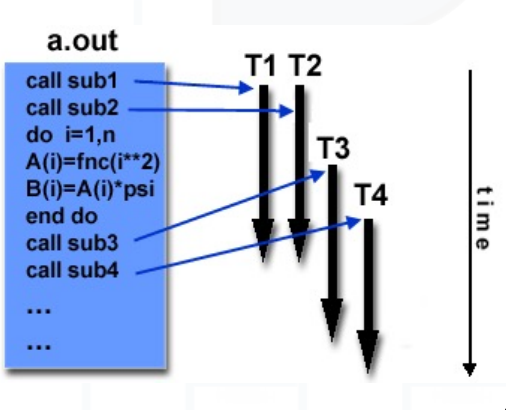
\includegraphics[width=0.7\linewidth]{img/modello-thread}
	\caption{modello con le thread.}
	\label{fig:modello-thread}
\end{figure}
Nel modello con le thread della programmazione parallela (figura \ref{fig:modello-thread}), un singolo processo può avere più percorsi di esecuzione simultanei. Forse l'analogia più semplice che può essere utilizzata per descrivere le thread, è il concetto di un singolo programma che include un numero di subroutine.
\begin{itemize}
	\item il programma principale a.out è pianificato per l'esecuzione dal sistema operativo. a.out carica ed acquisisce tutte le risorse utente e di sistema necessarie per l'esecuzione;
	\item a.out esegue del lavoro seriale e quindi crea una serie di thread che possono essere pianificate ed eseguite contemporaneamente dal sistema operativo;
	\item ogni thread ha dati locali, ma condivide anche tutte le risorse di a.out. Ciò consente di risparmiare il sovraccarico associato alla replica delle risorse di un programma per ciascuna thread. Ogni thread beneficia anche di una vista globale della memoria perché condivide lo spazio di memoria di a.out;
	\item il lavoro di una thread può essere meglio descritto come una subroutine all'interno del programma principale. Qualsiasi thread può eseguire qualsiasi subroutine contemporaneamente agli altri thread.
	\item le thread comunicano tra loro attraverso la memoria globale (in cui gli indirizzi vengono aggiornati). Ciò richiede costrutti di sincronizzazione per garantire che più di un thread non aggiorni lo stesso indirizzo globale in qualsiasi momento;
	\item le thread possono nascere e morire, ma a.out rimane presente per fornire le risorse condivise necessarie fino al completamento dell'applicazione.
\end{itemize}

\subsubsection{Implementazione del modello dei thread} Le thread sono comunemente associate ad architetture di memoria condivisa e a sistemi operativi. Dal punto di vista della programmazione, le implementazioni delle thread comprendono comunemente:
\begin{itemize}
	\item una libreria di subroutine chiamate dal codice sorgente parallelo \item un insieme di direttive del compilatore incorporate nel codice sorgente seriale o parallelo.
\end{itemize}
In entrambi i casi, il programmatore è responsabile della determinazione di tutto il parallelismo.

Le implementazioni threaded non sono nuove nell'informatica. Storicamente, i fornitori di hardware hanno implementate le proprie versioni proprietarie delle thread, che differivano sostanzialmente l'una dall'altra, rendendo difficile per i programmatori sviluppare applicazioni threaded portatili.

Gli sforzi di standardizzazione non correlati hanno portato a due implementazioni molto diverse delle thread:
\begin{enumerate}
	\item thread POSIX: sono specifiche del linguaggio C; sono comunemente indicate come \textit{Pthreads}; molti venditori di hardware le forniscono in aggiunta alle loro implementazioni proprietarie; il parallelismo è molto esplicito;
	\item OpenMP: è basato sulle direttive del compilatore; può utilizzare il codice seriale; definito e approvato congiuntamente da un gruppo di importanti fornitori di hardware e software per computer; è disponibile nelle implementazioni C/C++ e Fortran; è molto facile e semplice da usare: prevede il "parallelismo incrementale".
\end{enumerate}
\subsection{Modello di trasmissione dei messaggi}
\begin{figure}[th]
	\centering
	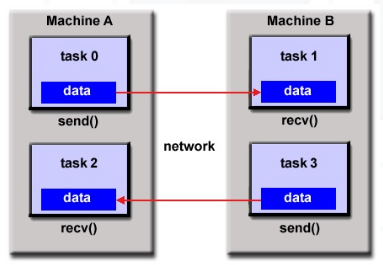
\includegraphics[width=0.7\linewidth]{img/modello-trasmissione-messaggi}
	\caption{modello di trasmissione dei messaggi.}
	\label{fig:modello-trasmissione-messaggi}
\end{figure}
Il modello di trasmissione dei messaggi (figura \ref{fig:modello-trasmissione-messaggi}) dimostra le seguenti caratteristiche:
\begin{itemize}
	\item una serie di task che usano la propria memoria locale durante la computazione. Tasks multipli possono risiedere fisicamente sulla stessa macchina e su un numero arbitrario di macchine;
	\item i task comunicano attraverso l'invio e la ricezione di messaggi;
	\item il trasferimento dei messaggi di solito richiede l'esecuzione di operazioni cooperative da parte di ciascun processo. Ad esempio, un'operazione di invio deve avere un'operazione di ricezione corrispondente.
\end{itemize}

\subsubsection{Implementazione del modello di passaggio dei messaggi} Dal punto di vista della programmazione, le implementazioni dello scambio di messaggi comprendono comunemente una libreria di subroutine incorporate nel codice sorgente. Il programmatore è responsabile di tutto il parallelismo. Nel 1992 è stato formato il Forum MPI con l'obbiettivo primario di stabilire un'interfaccia standard per le implementazioni dello scambio di messaggi. MPI è ora lo standard industriale "de facto" per lo scambio di messaggi.

Per le architetture a memoria condivisa, le implementazioni MPI solitamente non utilizzano una rete per le comunicazioni delle attività. Usano la propria memoria condivisa per motivi di prestazioni.

\subsection{Modello data parallel}
\begin{figure}[th]
	\centering
	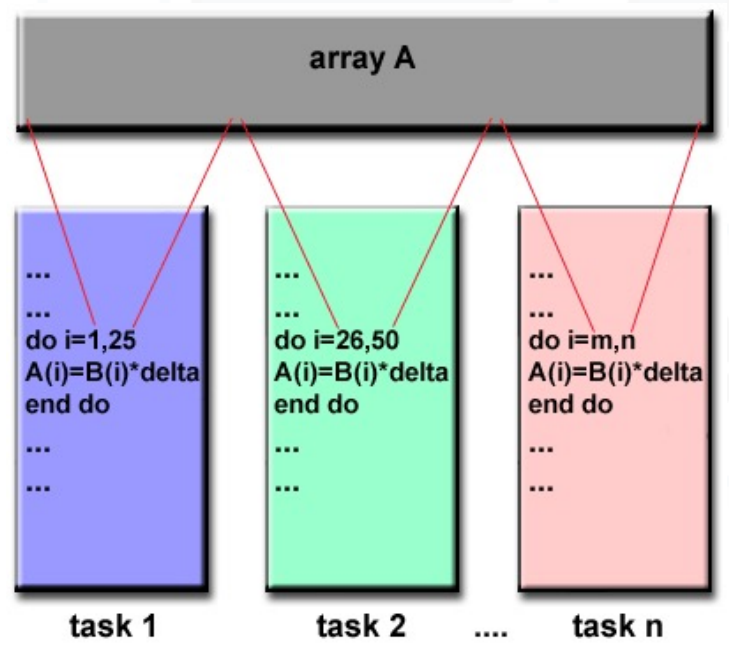
\includegraphics[width=0.7\linewidth]{img/modello-parallelo-dei-dati}
	\caption{modello data parallel.}
	\label{fig:modello-parallelo-dei-dati}
\end{figure}
Il modello data parallel (figura \ref{fig:modello-parallelo-dei-dati}) ha le seguenti caratteristiche:
\begin{itemize}
	\item la maggior parte del lavoro si concentra sull'esecuzione di operazioni su un set di dati. Il set è generalmente organizzato in una \textbf{struttura  dati comune}, ad esempio un array o un cubo;
	\item una serie di attività lavora collettivamente sulla stessa struttura dati, tuttavia, ogni attività funziona su una partizione diversa della stessa struttura dati;
	\item le attività eseguono la stessa operazione sulla loro partizione di lavoro, ad esempio "aggiungi 4 a ogni elemento dell'array";
	\item nelle architetture a memoria condivisa, tutte le attività possono avere accesso alla struttura dei dati attraverso la memoria globale. Nelle architetture di memoria distribuita la struttura dei dati è suddivisa e risiede come "chunks" (ovvero "pezzi") nella memoria locale di ciascun task.
\end{itemize}

\subsubsection{Implementazione del modello data parallel} La programmazione con il modello data parallel viene solitamente compiuta scrivendo un programma con costrutti data parallel. I costrutti possono essere chiamati tramite subroutine di una libreria che supporta data parallel o attraverso direttive per un compilatore data parallel.

Le implementazioni più comuni sono:
\begin{itemize}
	\item HPF (High Performance Fortran);
	\item direttive di compilatore;
\end{itemize}

\subsection{Modello ibrido} È un modello in cui possono essere combinati due o più modelli di programmazione parallela. Un esempio comune è di combinare il MPI (Message Passing Model) con il modello delle thread (thread POSIX) o in alternativa il modello della memoria condivisa (OpenMP).

Un altro esempio comune di modello ibrido consiste nel combinare i dati in parallelo con lo scambio di messaggi.
\subsection{Modello SPMD (Single Program Multiple Data)} SPMD è in realtà un modello di programmazione di "alto livello" che può essere costruito su qualsiasi combinazione dei modelli di programmazione parallela precedentemente menzionati. Un singolo programma viene eseguito da tutti i task contemporaneamente. In qualsiasi momento, le attività possono eseguire le stesse o differenti istruzioni all'interno dello stesso programma (figura \ref{fig:spmd}).
\begin{figure}[th]
	\centering
	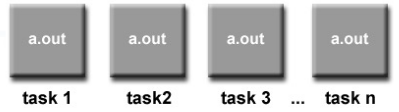
\includegraphics[width=0.7\linewidth]{img/SPMD}
	\caption{modello SPMD.}
	\label{fig:spmd}
\end{figure}
A differenza di SIMD (Single Instruction Multiple Data), nel SPMD, più processori autonomi eseguono simultaneamente lo stesso programma in punti indipendenti, anziché in unico \textbf{lockstep} che SIMD impone su dati diversi.\footnote{I sistemi lockstep sono sistemi informatici tolleranti agli errori che eseguono lo stesso insieme di operazioni contemporaneamente in parallelo.} Con SPMD, le attività possono essere eseguite per CPU general purpose; SIMD richiede processori vettoriali per manipolare i flussi di dati. SPMD è una sottocategoria di MIMD.

I programmi SPMD di solito hanno la logica necessaria programmata al loro interno per consentire a diversi task di fare una fork o di eseguire condizionatamente solo quelle parti del programma per cui sono state ideate. Cioè, le attività non devono necessariamente eseguire l'intero programma, ma solo una sua parte.

\subsection{Modello MPMD (Multiple Program Multiple Data)} 
\begin{figure}[th]
    \centering
    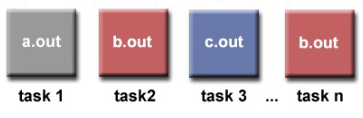
\includegraphics[width=0.75\linewidth]{img/mpmd.png}
    \caption{Enter Caption}
    \label{fig:enter-label}
\end{figure}
Come SPMD, MPMD (figura \ref{fig:enter-label}) è in realtà un modello di programmazione di "alto livello" che può essere costruito su qualsiasi combinazione dei modelli di programmazione parallela precedentemente menzionati. Applicazioni MPMD hanno tipicamente più file oggetti eseguibili (programmi). Mentre l'applicazione viene eseguita in parallelo, ciascun task può eseguire lo stesso o un altro programa. Tutti i task potrebbero eseguire dati diversi.
	\section{Valutazione delle performance}
La valutazione delle performance viene fatta per due motivi:
\begin{itemize}
    \item dal punto di vista dell'\textbf{utente} per ridurre il tempo di risposta. È nota anche come \textbf{tempo di esecuzione} o \textbf{latenza}. Definita come il tempo trascorso dall'inizio al completamento del compito o lavoro;

\item dal punto di vista del \textbf{sistema} per aumentare il \textbf{throughput}, ovvero la quantità totale di lavoro svolto in un dato intervallo di tempo, a volte chiamato \textbf{larghezza di banda}.

\end{itemize}

Lo speedup è definito come il rapporto tra il tempo di esecuzione di due programmi:
\begin{equation*}
	n=\frac{execTime_y}{execTime_x}
	=\frac{\frac{1}{\textsc{Performance}_y}}{\frac{1}{\textsc{Performance}_x}}=\frac{\textsc{Performance}_x}{\textsc{Performance}_y}
\end{equation*}
e misura il miglioramento delle prestazioni. \textbf{Nota:} il tempo di esecuzione è \textit{inversamente proporzionale} alle performance. Di solito $execTime_y$ viene sostituito dal tempo di esecuzione della versione sequenziale di un programma $P$ e $execTime_x$ con la sua versione parallelizzata.

Le misurazioni delle performance possono essere fatte a diversi livelli (considerando solo l'architettura hardware, una sua parte, o una parte di codice, o un intero programma, oppure tutto l'insieme) sfruttando funzionalità contenute in una \textbf{benchmark suite} (un insieme di tool di benchmark, come i \textbf{kernels} che sono piccoli pezzi di codice chiave presi da applicazioni reali, oppure i \textbf{toy programs} che contengono programmi, solitamente lunghi 100 linee di codice, che implementano algoritmi come la moltiplicazione tra matrici, il quicksort, e così via. Vi sono poi i \textbf{benchmark sintetici}, ovvero programmi ideati per simulare il comportamento delle applicazioni reali (come il Linpak, e il Dhrystone). La \textbf{SPEC} (Standard Performance Evaluation Corporation) è un consorzio senza scopo di lucro che stabilisce, mantiene e approva benchmark e strumenti standardizzati per valutare le prestazioni per la nuova generazione di sistemi informatici. SPEC sviluppa suite di benchmark e inoltre esamina e pubblica i risultati presentati dalle nostre organizzazioni membri e da altri licenziatari di benchmark.

Per comparare le performance di un componente hardware può essere consultata una \textbf{tabelle delle performance} dei modelli disponibili in commercio. Le informazioni più importanti riguardano i benchmark per completare un particolare task e il costo del componente hardware.

\subsection{Principio quantitativo} Per aumentare lo speedup è necessario concentrare le energie sul codice che viene eseguito più frequentemente, piuttosto che quello eseguito più raramente.

Un importante riferimento a tal proposito, è la \textbf{legge di Amdahl}.

\vspace{.5cm}
\begin{tcolorbox}[title=Legge di Amdahl]
    \textit{"Il miglioramento delle prestazioni di un sistema che si può ottenere ottimizzando una certa parte del sistema è limitato dalla frazione di tempo in cui tale parte è effettivamente utilizzata"}.
\end{tcolorbox}
\vspace{.5cm}

\subsubsection*{Legenda}
\begin{table}[th]
	\centering
	\begin{tblr}{|c|c|}
		\hline
		$e_n$ & execution time new
		\\\hline
		$e_o$ & execution time old
		\\\hline
		$f_i$ & fraction improved
		\\\hline
		$s_i$ & speedup improved
		\\\hline
		$s_g$ & speedup global
		\\\hline
	\end{tblr}
\end{table}

Di seguito con $f_i \le 1$ (\textit{"fraction improved"}) viene indicata la frazione del tempo di esecuzione della macchina originale (o del codice originale) che può essere modificata per trarre vantaggio dalle migliorie, mentre con $s_i \ge 1$ (\textit{"speedup improved"}) viene indicato il miglioramento ottenuto da un una modalità di esecuzione più veloce.
\begin{align}
    e_n &= e_o \cdot \left((1-f_i) + \frac{f_i}{s_i} \right) \label{eqn:execution-time-new} \\
    s_g &= \frac{e_o}{e_n}= \frac{1}{(1-f_i)+ \frac{f_i}{s_i}}\label{eqn:speedup-global}
\end{align}
Se un miglioramento può essere usato solo per una frazione dell'intero task:
\begin{equation}
    s_g = \frac{1}{(1-f_i)+\frac{f_i}{s_i}} \fcolorbox{red}{white}{$\le \frac{1}{(1-f_i)}$} \label{eqn:speedup-global-with-limit}
\end{equation}


Lo \textbf{speedup globale} $s_g$ è uguale a $ \frac{1}{(1-f_i)+\frac{f_i}{s_i}}$ dove $1-f_i$ è la frazione non parallelizzabile, $f_i$ è la frazione parallelizzabile e $s_i$ è lo speedup che si ottiene dalla porzione parallelizzabile di codice. Lo speedup globale massimo, nel riquadro rosso (equazione \ref{eqn:speedup-global-with-limit}) si ottiene facendo tendere la $s_i$ all'infinito: \[\lim_{s_i \to \infty}{\frac{f_i}{s_i}} = 0\]
\begin{exercise}
	Si consideri un miglioramento di 10 volte più veloce della macchina originale (o del codice) ma che può essere applicato solo per il 40\% del tempo. Qual'è il guadagno totale?
\end{exercise}
\begin{solution}
	Traendo i dati dal problema, si ottiene che lo $s_i = 10$ e che $f_i = 40\% = 0,4$. Sostituendo alla formula \ref{eqn:speedup-global} si ottiene
	\begin{equation*}
		s_g = \frac{1}{(1-0.4)+\frac{0.4}{10}} = \frac{1}{0.6+0.04} = \frac{1}{0.64} = \frac{100}{64} = 1.56
	\end{equation*}

	Lo speedup ottenuto è di 1.56.
\end{solution}

\begin{exercise}
	Si consideri una CPU che è stata aggiornata per avere i seguenti cambiamenti:
	\begin{enumerate}
		\item aumentare la velocità di un fattore pari a 5 senza interessare le performance del sistema I/O;
		\item il costo è 5 volte superiore al precedente;
		\item la CPU può essere utilizzata per il 50\% del tempo totale, mentre il rimanente viene impiegato per operazioni di I/O;
		\item il costo della CPU è $\frac{1}{3}$ del costo della macchina.
	\end{enumerate}
	Questo investimento, è conveniente?
\end{exercise}
\begin{solution}
	Lo $s_i = 5$, la $f_i = 50\% = 0.5$. Lo speedup globale è:
	\begin{equation*}
		s_g = \frac{1}{(1-0.5)+\frac{0.5}{5}}=\frac{1}{0.5+0.1} = \frac{10}{6} = 1.67
	\end{equation*}
	il costo è aumentato di:
	\begin{equation*}
		c = 1 \cdot \frac{2}{3} + 5 \cdot \frac{1}{3} =\frac{7}{3} = 2.33
	\end{equation*}
	Dato che il costo è superiore al rendimento ottenuto $ c = 2.33 >  s_g = 1.67 $ non è conveniente fare l'aggiornamento del processore.
\end{solution}

\begin{exercise}
	Si vuole riscrivere un programma su un'architettura MIMD con 100 processori. L'obbiettivo è di ridurre il tempo di esecuzione di 80 volte rispetto a quello precedente su un'architettura SISD. Qual'è la frazione del programma originale che può restare sequenziale?
\end{exercise}
\begin{solution}
	L'impostazione del problema è diversa dai precedenti. Il tempo di esecuzione della soluzione parallela è 80 volte più veloce di quella sequenziale. Si può osservare che il tempo totale è dato dalla somma del tempo di esecuzione della parte sequenziale e di quella parallela.
	\begin{align*}
		T&=\frac{T_{\textsc{sisd\textsubscript{\textsc{par}}}}}{\#\textsc{processori}}+\textsc{T\textsubscript{SISD}\textsubscript{\textsc{nonpar}}}\\
		&=\frac{T\textsubscript{\textsc{sisd}}\cdot \%\textsc{par}}{\#\textsc{processori}}+T_\textsc{sisd}\cdot\underbrace{ (1-\% par) }_{\%\textsc{nonpar}}
	\end{align*}
	La percentuale parallelizzabile è dell' $80\%$ rispetto al tempo iniziale ($T_\textsc{SISD}$).  Il numero di processori è $100$. Per semplicità si imposta ad $x=\% par$, ovvero la percentuale cercata.
	Sostituendo i dati nella formula:
	\begin{align*}
		\frac{\cancel{T_\textsc{sisd}}}{80}&=T_{\cancel{\textsc{sisd}}}\cdot \left(\frac{x}{100}+\underbrace{(1-x)}_{\textsc{\% nonpar}}\right)\\
		\frac{1}{80} &=  \frac{x}{100} + (1-x)\implies \frac{x+100-100\, x}{100}=\frac{1}{80}
		 \\ &\implies x = \left(\frac{5}{4}-100\right)\cdot\frac{1}{-99}\implies x = \frac{-395}{4}\cdot \frac{1}{-99}=0.997\\ &\implies x = 99.7\%
	\end{align*}
\end{solution}

\begin{exercise}
	Sapendo che il calcolo parallelo è 20 volte più veloce rispetto all'originale (sequenziale), calcolare:
	\begin{itemize}
		\item  la percentuale di parallelismo è la porzione di tempo impiegata utilizzando la modalità di esecuzione SIMD.
		\item Disegna un grafico per rappresentare il miglioramento delle prestazioni come percentuale del calcolo eseguito in modalità SIMD.
		\item  Quale percentuale di parallelismo è necessaria per ottenere un miglioramento delle prestazioni pari a 2? Quale per raggiungere la metà del miglioramento massimo?
	\end{itemize}
\end{exercise}
\begin{solution}
	Lo speedup che si ottiene è il seguente. Si pone $x=\% par$
	\begin{align*}
		\textsc{speedup} = \frac{1}{(1-x)+\frac{x}{\text{speedup par.}}} = \frac{1}{(1-x)+\frac{x}{20}} = \frac{20}{20-19 \, x}
	\end{align*}
	Il grafico è il seguente.
	\begin{figure}[ht]
		\centering
		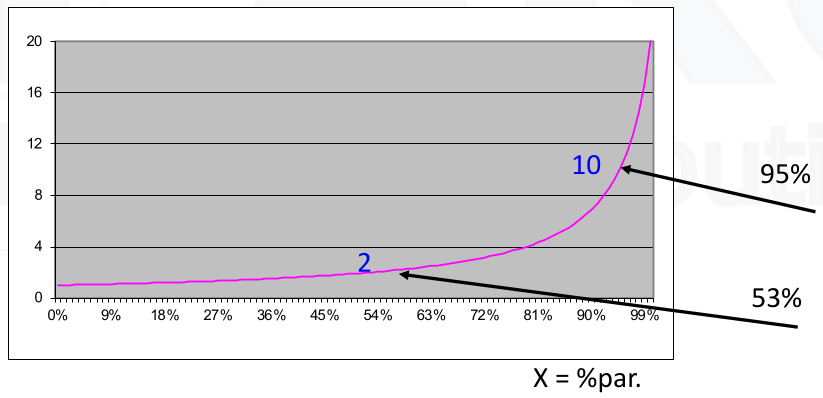
\includegraphics[width=0.7\linewidth]{img/graph-ex4}
		\caption{grafico dello speedup.}
		\label{fig:graph-ex4}
	\end{figure}
\end{solution}
Si consideri ora lo stesso esercizio ma con questi dati.
\begin{exercise}
	La percentuale di parallelismo raggiungibile è del 70\%. Ci sono due alternative.
	\begin{enumerate}
		\item Raddoppiare la velocità della modalità SIMD (è molto costoso)
		\item Aumentare la percentuale di parallelismo concentrandosi sul compilatore.
	\end{enumerate}
	Quale \textbf{aumento} della percentuale di parallelismo è necessario per ottenere lo stesso guadagno di prestazioni?
\end{exercise}
\begin{solution}
	Lo speedup originale si ottiene facendo
	\begin{equation*}
		\textsc{speedup orig}[20 \cdot 70 \%] = \frac{1}{(1-0.7)+\frac{0.7}{20}} = \frac{20}{20-14+0.7}=2.9851
	\end{equation*}
	Raddoppiando la velocità della modalità SIMD
	\begin{equation*}
		\textsc{speedup hw}[20 \cdot 70\%] = \frac{1}{(1-0.7)+\frac{0.7}{40}}=\frac{40}{40-28+0.7}=3.1496
	\end{equation*}
	Lo speedup adottando il compilatore è ovviamente parametrico, perché ci si sta chiedendo quale sia la percentuale necessaria per ottenere lo stesso guadagno di prestazioni, ed è il seguente.
	\begin{equation*}
		\textsc{speedup compiler}[20\cdot x\%] = \frac{1}{(1-x)+\frac{x}{20}}=\frac{20}{20-19\, x}
	\end{equation*}
	Si pone dunque
	\[\textsc{speedup compiler}= \textsc{speedup hw}\]
	ovvero
	\begin{equation*}
		\frac{20}{20-19\, x} = 3.1496 \implies x = 0.7184
	\end{equation*}
	Dunque è sufficiente una parallelizzazione del 71.84\%.
\end{solution}
\begin{exercise}
	Si consideri un'architettura basata su cache. La memoria cache è 5 volte più veloce della memoria principale. La cache è usata per il 90\% del tempo. Ci si chiede quale sia lo speedup con e senza cache.
\end{exercise}
\begin{solution}
	Lo speedup è il seguente.
	\begin{equation*}
		\textsc{speedup} = \frac{1}{(1-x)+\frac{x}{\textsc{speedup con cache}}} = \frac{1}{(1-0.9)+\frac{0.9}{5}}=\frac{1}{0.28}\approx 3.6
	\end{equation*}
	Si conclude che l'architettura basata su cache è più veloce di 3.6 volte la velocità della stessa architettura senza cache.
\end{solution}
%%%%%%%%%%%%%%%%%%%%%%%%%%%%%%%%%%%%%%%%%%%%%%%%%%%%%%%%%%%%%%%%%%%%%%%%

\subsection{Tempo di esecuzione} Il tempo di esecuzione viene usato per misurare le performance di un computer: l'architettura che esegue la stessa quantità di lavoro in meno tempo è la più veloce. Il \textbf{tempo di risposta} rappresenta la latenza per completare un task e include accessi al disco, gli accessi alla memoria e le operazioni di input/output. Il \textbf{CPU time} ovvero il tempo impiegato per svolgere operazioni di CPU (cicli di clock per eseguire il codice interessato, per operazioni di sistema -- ad esempio per la stampa a video -- mentre non è considerato CPU time il tempo speso per attendere dati o istruzioni accedendo in memoria perché è un tempo di attesa. 
Il CPU time è calcolato come segue:
\begin{align*}
\text{CPU\textsubscript{\textsc{time}}} &= \text{Cicli di clock della CPU per una task} * \text{tempo di un ciclo di clock}\\
&= \frac{\text{Cicli di clock della CPU per una task}}{\text{Frequenza di clock}}
\end{align*}

I Cicli di clock medi per istruzione (CPI) medi vengono calcolati come segue:
\begin{align*}
\text{CPI} &= \frac{\text{Cicli di clock della CPU per una task}}{\text{Numero di istruzioni}}\\
\text{CPU\textsubscript{\textsc{time}}} &= \text{N di istruzioni} * \text{CPI} * \text{durata di un ciclo di clock}\\
&= \frac{\text{N di istruzioni} * \text{CPI}}{\text{Frequenza di clock}}\\
T\textsubscript{\textsc{{cpu}}} &= \text{CI}* \text{CPI} * T\textsubscript{\textsc{clock}} = \frac{\text{CI} * \text{CPI}}{f\textsubscript{\textsc{{clock}}}}
\end{align*}

La relazione tra le varie metriche è visibile di seguito:
\begin{align*}
    \frac{\text{istruzioni}}{\text{task}} * \frac{\text{cicli di clock}}{\text{istruzione}} * \frac{\text{secondi}}{\text{cicli di clock}}= \frac{\text{secondi}}{\text{task}} = \text{CPU time}
\end{align*}

Il tempo di CPU dipende da 3 parametri:
\begin{itemize}
    \item \textbf{Ciclo di clock (o frequenza)}: dipende dalla tecnologia, quindi l'unico modo per migliorare questo parametro consiste nel sostituire l'architettura.
    \item \textbf{CPI}: è il numero di cicli di clock medio per istruzione. Dipende dall'organizzazione dell'architettura e dall'istruction set architecture (ISA), che è l'insieme delle istruzioni che vengono gestite dall'architettura; se queste sono complesse, richiedono generalmente più cicli di clock.
    \item \textbf{Numero di istruzioni}: il numero di istruzioni usate da un programma dipende dall'instruction set architecture e dalla tecnologia del compilatore. Un buon compilatore permette idealmente di avere un codice finale con meno istruzioni (ovviamente un fattore importante rimane la capacità del programmatore). Questo parametro è quello in cui è più fattibile intervenire.
\end{itemize}

Il numero totale di cicli di clock per una task si calcola come segue:
\begin{align*}
    \text{Cicli di clock della CPU} = \sum^n_{i=1} (CPI_i * I_i)
\end{align*}
dove:
\begin{itemize}
    \item $I_i$ rappresenta il numero di volte in cui l'istruzione $I$ è stata eseguita in una task;
    \item $CPI_i$ rappresenta il numero medio di cicli di clock spesi per una generica istruzione.
\end{itemize}

Date queste misure, il CPU time può essere riscritto come:
\begin{align*}
    T_{CPU} = \sum^n_{i = 1} (CPI_i * I_i) * T_{CLOCK}
\end{align*}

\begin{exercise}
	Si supponga di avere effettuato le seguenti  misurazioni.
	\begin{itemize}
		\item Frequenza delle operazioni in virgola mobile (incluse le FPSQR) = 25\%
		\item CPI medio delle operazioni in virgola mobile = 4.0
		\item Frequenza delle operazioni FPSQR (radice quadrata in virgola mobile) = 2\%
		\item CPI delle operazioni FPSQR = 20.0
	\end{itemize}
	Ci sono due possibilità:
	\begin{enumerate}
		\item Decrementare la CPI del FPSQR a 2
		\item Decrementare il CPI medio di tutte le operazioni FP (floating point) di 2.5
	\end{enumerate}
	Comparare le due alternative in termini di performance complessive.
\end{exercise}
\begin{solution}
	Si ricava il CPI originale
	\begin{equation*}
		\textsc{cpi}_{\textsc{orig}}=(0.25\cdot 4)+(0.75 \cdot 1.33)=2.00
	\end{equation*}
	Si può calcolare il CPI per l'FPSQR migliorato, sottraendo i cicli risparmiati dal CPI originale:
	\begin{align*}
		\textsc{cpi}_1 &= \textsc{cpi}_{\textsc{orig}}-2\% \cdot \left(\textsc{cpi}_{\textsc{old\_fspqr}}-\textsc{cpi}_\textsc{new\_fspq\_only}\right)\\&=2.00-2\%\cdot(20-2)=1.64
	\end{align*}
	È possibile calcolare il CPI per il miglioramento di tutte le istruzioni FP e allo stesso modo sommando i CPI delle istruzioni FP e non FP. Utilizzando quest'ultimo metodo si ottiene:
	\begin{equation*}
		\textsc{cpi}_2 = \left(75\% \cdot 1.33\right)+(25\% \cdot 2.5) = 1.625
	\end{equation*}
	Dato che il CPI del miglioramento complessivo delle istruzioni FP è leggermente più basso, le sue prestazioni saranno leggermente migliori. Nello specifico, il miglioramento delle prestazioni complessive delle istruzioni FP è:
	\begin{align*}
			\textsc{speedup}_2 = \frac{\textsc{cpu\textsubscript{time\textsubscript{orig}}}}{\textsc{cpu\textsubscript{time\textsubscript{2}}}}= \frac{\textsc{ic}\cdot \textsc{clock\textsubscript{cycle}}\cdot \textsc{cpi}\textsubscript{\textsc{orig}}}{\textsc{ic}\cdot \textsc{clock\textsubscript{cycle}}\cdot \textsc{cpi}\textsubscript{\textsc{2}}}=\frac{\textsc{cpi\textsubscript{orig}}}{\textsc{cpi\textsubscript{2}}}=\frac{2.00}{1.625}=1.23
	\end{align*}
\end{solution}
\begin{exercise}
	L'architettura inizialmente dispone solo di istruzioni di caricamento e memorizzazione per accedere alla memoria. Tutte le altre operazioni lavorano nei registri (architettura L/S). Il riassunto delle istruzioni è riportato nella tabella.
	\begin{table}[ht]
		\centering
		\begin{tabular}{|l|c|c|}
			\hline
			& \textbf{Frequenza}&\textbf{Cicli di clock}
			\\\hline
			ALU & 43\% & 1
			\\\hline
			Load & 21\% & 2
			\\\hline
			Store & 12\% & 2
			\\\hline
			Branch & 24\% & 2
			\\\hline
		\end{tabular}
	\end{table}
	Si supponga che il 25\% delle operazioni dell'ALU utilizzi un operando specificamente caricato, che non è più utile per le operazioni successive. Viene proposto di aggiornare il set di istruzioni avendo uno degli operandi di origine in memoria. Queste nuove operazioni reg-mem hanno un numero di cicli di clock pari a 2 e richiedono 3 cicli di clock per i salti, senza modificare il periodo del ciclo di clock. Questa modifica può migliorare le prestazioni della CPU?
\end{exercise}
\begin{solution}
	Si ottiene $\textsc{cpi\textsubscript{old}}$
	\begin{equation*}
		\textsc{cpi\textsubscript{old}} = 0.43 \cdot 1 + 0.21 \cdot 2 + 0.12 \cdot 2 + 0.24 \cdot 2 = 1.57
	\end{equation*}
	Il tempo di $\textsc{cpi}\textsubscript{old}$ si ottiene come:
	\begin{equation*}
		\textsc{t\textsubscript{cpu\textsubscript{old}}} = \textsc{ci\textsubscript{old}} \cdot1.57 \cdot \textsc{t\textsubscript{clock\textsubscript{old}}}
	\end{equation*}
	il $\textsc{cpi}\textsubscript{new}$ è:
	\begin{equation*}
		\textsc{cpi\textsubscript{new}} = \frac{\splitfrac{(0.43-(0.25 \cdot 0.43))\cdot 1+(0.21-(0.25\cdot 0.43))\cdot 2+}{ +(0.25\cdot 0.43)\cdot 2+ 0.12 \cdot 2 + 0.24 \cdot 3}}{1-(0.25 \cdot 0.43)}
	\end{equation*}
	Si ricava il$\textsc{t\textsubscript{cpu\textsubscript{new}}}$:
	\begin{equation*}
		\textsc{t\textsubscript{cpu\textsubscript{new}}}=(0.893\cdot \textsc{ci\textsubscript{old}})\cdot(1.908 \cdot \textsc{t\textsubscript{clock\textsubscript{old}}})=1.703 \cdot \textsc{ci\textsubscript{old}} \cdot \textsc{t\textsubscript{clock\textsubscript{old}}}
	\end{equation*}
	L'introduzione delle istruzioni reg-mem non compensa l'aumento del tempo di esecuzione dei salti.
\end{solution}
\subsection{MIPS e GIPS}
Con le sigle MIPS e GIPS si intendono rispettivamente milioni di microistruzioni per secondo e miliardi di microistruzioni per secondo, dove:
\begin{align*}
    MIPS &= \frac{\text{N di istruzioni}}{\text{Tempo di esecuzione} * 10^6}\\
    &= \frac{\text{frequenza di clock}}{CPI * 10^6}
\end{align*}

Il tempo di esecuzione diventa:
\begin{align*}
    \text{Tempo di esecuzione} = \frac{\text{N di istruzioni}}{MIPS * 10^6}
\end{align*}
\
Poiché MIPS rappresenta la frequenza di operazioni per unità di tempo, le performance per la macchina più veloce cha ha alti valori MIPS può essere specificata come l'inversa del tempo di esecuzione. Il vantaggio del MIPS è che è semplice da capire: le macchine più veloci hanno valori MIPS più alti. 

La metrica MIPS presenta comunque una serie di problematiche:
\begin{itemize}
    \item Il valore dipende dall'instruction set, quindi è difficile da comparare con macchine che hanno diversi instruction set;
    \item Varia in base al programma considerato;
    \item Varia in modo inversamente proporzionale alla performance.
\end{itemize}

La limitazione principale di questa misura è che non considera il tipo di istruzioni eseguite. Ad esempio, le operazioni su interi sono generalmente più







Se ci interessa misurare nello specifico le performance relative alle operazioni floating-point possiamo utilizzare la metrica GFLOPS, che sta per \textbf{billion of FP instructions per second} (dove FP indica le operazioni floating-point):
\begin{align*}
    GFLOPS = \frac{\text{N di \textbf{operazioni} FP in un programma}}{\text{Tempo di esecuzione} * 10^9}
\end{align*}

Ovviamente questa metrica non può essere usata in contesti diversi da quelli legati alle operazioni FP. Essendo basata su operazioni piuttosto che istruzioni, i FLOPS sono concepiti per essere un buon metodo di confronto tra le varie architetture. L'ipotesi è che stesso programma, lanciato su differenti architetture, esegue un diverso numero di istruzioni, ma lo stesso numero di operazioni floating-point. Le operazioni FP non sono considerate tra diverse architetture; il GFLOPS cambia cambiando il rapporto tra le operazioni intere e FP oppure cambiando il mix di operazioni FP veloci e lente.

Il \textbf{Normalized GFLOPS} prevede di associare un bias, con funzione di peso, ad ogni operazione FP, come mostrato in figura \ref{fig:normalized-gflops}.
\begin{figure}[th]
	\centering
	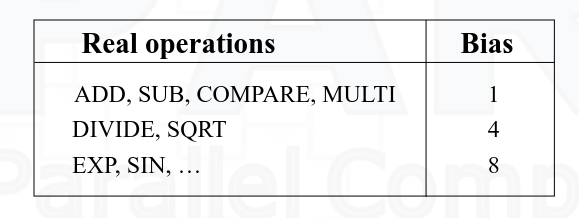
\includegraphics[width=0.7\linewidth]{img/normalized-gflops.png}
	\caption{Esempio di bias per operazioni FP.}
	\label{fig:normalized-gflops}
\end{figure}

Un frammento di codice con operazioni un'operazione ADD, una DIVIDE e una SIN, si calcola avere 12 operazioni FP normalizzate.
\newpage
\begin{exercise}
	Il programma Spice viene eseguito su una DECstation 3100 in 0,094 secondi. Il numero di operazioni in virgola mobile eseguite dal programma è riportato nella tabella.
	\begin{table}[ht]
		\centering
		\scriptsize
		\begin{tabular}{|l|r|}
			\hline
			addD & 25,999,440
			\\\hline
			subD & 18,266,439
			\\\hline
			mulD & 33,880,810
			\\\hline
			divD & 15,682,333
			\\\hline
			compareD & 9,745,930
			\\\hline
			negD & 2,617,846
			\\\hline
			absD & 2,195,930
			\\\hline
			convertD & 1,581,450
			\\\hline
			\textbf{totale} & \textbf{109,970,178}
			\\\hline
		\end{tabular}
	\end{table}
	Calcolare:
	\begin{itemize}
		\item I GFLOPS del programma.
		\item I GFLOPS normalizzati.
	\end{itemize}
\end{exercise}
\begin{solution}
	\begin{align*}
		\textsc{ci\textsubscript{ott}} &= \textsc{ci\textsubscript{non ott}}\cdot \left[(1-0.3)\cdot \left(1-\frac{1}{3}\right)\right]=0.9 \cdot \textsc{ci\textsubscript{non ott}}\\
		\textsc{ci\textsubscript{ott}} &= \textsc{cpi\textsubscript{non ott}}=1\\
		\textsc{t\textsubscript{\textsc{clock\textsubscript{ott}}}} &= 1.05 \cdot \textsc{t\textsubscript{\textsc{clock\textsubscript{non ott}}}}\\
		\textsc{t\textsubscript{cpu\textsubscript{ott}}} &= 0.9 \cdot \textsc{ci\textsubscript{non ott}} \cdot \textsc{cpi\textsubscript{\textsc{non ott}}}\cdot\textsc{t\textsubscript{clock\textsubscript{non ott}}}\\
		&=0.945 \cdot \textsc{ci\textsubscript{non ott}}\cdot \textsc{cpi\textsubscript{non ott}}\cdot \textsc{t\textsubscript{clock\textsubscript{non ott}}}\\
		&= 0.945 \cdot \textsc{t\textsubscript{cpu\textsubscript{non ott}}}
	\end{align*}
\end{solution}















    \section{Prospettive sulla programmazione parallela}
Uno degli aspetti più importante è analizzare il problema e capire se può essere parallelizzato. La parallelizzazione del codice parta a dei miglioramenti delle performance solo se il workload (peso computazionale) è non indifferente.


Partiamo con un po' di definizioni:
\begin{itemize}
    \item Task: arbitrario pezzo di lavoro/sequenza di codice in una computazione parallela. Viene eseguito sequenzialmente, la concorrenza si ha solo tra le task;
    una task è una sequenza di istruzioni che andiamo a identificare, è una parte del programma.
    \item Processo/thread: entità astratta che performa le task assegnate ai progetti. I processi comunicano e si sincronizzano per eseguire le lo task.
    \item Processore: motore fisico sul quale si eseguono i processi. Più thread possono essere eseguiti sullo stesso processore, un thread non può essere eseguita su più processori.
\end{itemize}

\subsection{Step per creare un programma parallelo}
Possiamo identificare 4 passi nella creazione di un programma parallelo:
\begin{enumerate}
    \item Decomposizione della computazione in task -> parto dall'algoritmo risolutivo e identifico tutte le task che lo compongono (divido il problema in sottoproblemi);
    \item Assegnamento delle task ai processi (mappiamo le task identificate nelle thread disponibili); 
    \item Orchestrazione degli accessi ai dati, della comunicazione e della sincronizzazione -> si capisce come raggruppare i processi in unità da eseguire in parallelo;
    \item Mapping dei processi ai processori. Ovviamente, un processo non può essere assegnato a più unità di calcolo.
\end{enumerate}

Le fasi di \textbf{decomposizione} e \textbf{assegnamento} compongono la fase di partizionamento del problema (partiamo da un problema grosso e lo dividiamo su processi computazionale). Qui in pratica è dove identifichiamo il livello di parallelismo.

\subsubsection{Comprensione del problema/programma}
Il primo reale step da eseguire resta però il capire il problema e/o il programma. Se stiamo partendo da un programma sequenziale già scritto, dobbiamo per forza capire come funziona per poterlo parallelizzare, mentre nel caso del problema dobbiamo capire se questo è anche parallelizzabile. 
In generale quello che dobbiamo fare è:
\begin{enumerate}
    \item Identificare gli hotspot del programma: rappresentano le parti più "pesanti" del codice e sono solitamente identificati dopo aver fatto profiling\footnote{I tool di profiling eseguono il codice e, assieme al suo risultato, ritornano anche un report che può contenere: il numero di invocazioni a funzione per ogni funzione del codice, il tempo impiegato da ogni esecuzione di ogni funzione, quali parti del codice sono più usate, ...} e analisi delle performance (tramite appositi tool). Gli hotspot sono generalmente le sezioni in cui si concentra la parallelizzazione.
    \item Identificare i bottleneck del programma: rappresentano i punti del codice che sono più lente ad eseguire (come ad esempio le sezioni dedicate all'I/O). Una possibile strada che si può seguire per i bottleneck consiste nel trasferire la loro esecuzione sulla GPU, in modo da non dover rallentare la CPU. Possiamo quindi vedere due livelli di parallelismo: il primo dato dalla GPU che parallelizza la funzione, mentre il secondo dato dalla concorrenza di esecuzione di CPU e GPU.
    \item Identificare gli inibitori al parallelismo: analizzare il problema significa anche identificare gli inibitori del parallelismo, che sono quei fattori che impediscono di parallelizzare il codice. Generalmente, un inibitori dal parallelismo è la dipendenza delle task, dove il risultato di quella successiva dipende dal risultato di quella precedente.
\end{enumerate}

\underline{Esempio di problema parallelizzabile}: Calcolare l'energia potenziale per ciascuna delle diverse migliaia indipendenti Conformazioni di una molecola. Al termine, trova la conformazione energetica minima. Ogni conformazione molecolare è indipendentemente determinabile e il calcolo della conformazione energetica minima è parallelizzabile.
\\

\underline{Esempio di problema non-parallelizzabile}: Calcolare la serie di Fibonacci. Questo problema non è parallelizzabile in quanto il calcolo attuale dipende dai calcoli precedenti (il termine $k+2$ è dato dalla somma dei termini $k+1$ e $k$). 
\\



\subsubsection{Decomposizione}
Nella scomposizione andiamo ad identificare task sufficiente affinché ce ne sia abbastanza da poter tenere le thread, e i corrispondenti processori, sempre occupati. Questo significa che se abbiamo una macchina con 100 processori, che possono andare tutti in parallelo, dobbiamo avere un pool di task sufficientemente grande da poter tenere occupati tutti i processori anche nel momento in cui una delle task si blocca. Infatti capiterà che una task arrivi al punto in cui necessità di dati da un'altra task o di eseguire operazioni di I/O, restando quindi bloccata e lasciando inutilizzato il processore. Quello che vogliamo evitare è appunto il suo utilizzo, che possiamo evitare se disponiamo di un'altra task pronta ad essere eseguita appena un processore si libera. Dei core/processori lasciati in stallo (inutilizzati) ci ritroviamo con uno spreco di risorse.
Per farla semplice, ci serve un numero di task sufficiente a permetterci di rimpiazzare immediatamente quelle "bloccate" per evitare l'inutilizzo dei processori.

Esistono due modi per scomporre in task:
\begin{itemize}
    \item Scomposizione di dominio: prevede di scomporre i dati del problema, facendo lavorare poi ogni task su una porzione dei dati. Esistono vari modi di partizionare i dati, la soluzione migliore generalmente dipende dal modo in cui sono memorizzati i dati sul pc.

    I problemi, che siano monodimensionale che bidimensionali, possono essere scomposti, ad esempio, in blocchi o cicli (figure \ref{fig:domain-decomposition}). Un fattore importante da tenere presente è il bilanciamento del carico. se siamo sicuri che il tempo impiegato dalla prima thread sul blocco A corrisponde a quello impiegato dalla seconda thread sul blocco B e così via per il resto dei blocchi, allora abbiamo un carico bilanciato. Questo di solito è il caso per problemi lineari. Quando però abbiamo problemi più complessi, il carico di lavoro di una thread diventa imprevedibile. In questo caso potrebbe essere più ottimale aumentare i blocchi facendo in modo che il primo processore che si libera vada a prendere la successiva thread in attesa.
    \begin{figure}[th]
    	\centering
    	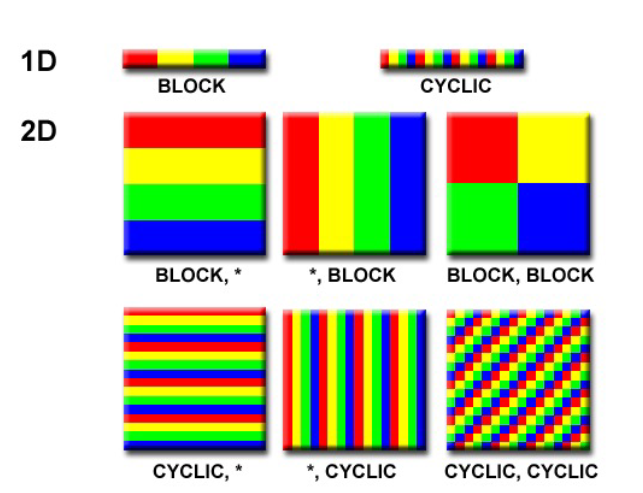
\includegraphics[width=0.7\linewidth]{img/domain-decomposition.png}
    	\caption{Esempio di decomposizione del dominio.}
    	\label{fig:domain-decomposition}
    \end{figure}

    \item Scomposizione funzionale: ci si concentra sull'elaborazione che deve essere fatta piuttosto che sui dati manipolati dalla computazione. Il problema è quindi scomposto rispetto al lavoro che deve essere fatto. Ogni task esegue parte del lavoro totale.
\end{itemize}

La scomposizione è compito del programmatore, che può essere supportato da tool automatici (campo di ricerca).

\underline{Esempio di parallelizzazione}
\\

Data un'immagine $NxN$ vogliamo:
\begin{itemize}
    \item Raddoppiare la luminosità di ogni pixel;
    \item Calcolare la media di tutti i pixel.
\end{itemize}

Una risoluzione sequenziale di questo problema costa un tempo totale di $2N^2$, con ogni step che ne costa $N^2$ (figure \ref{fig:esecuzione-sequenziale}). 
\begin{figure}[th]
	\centering
	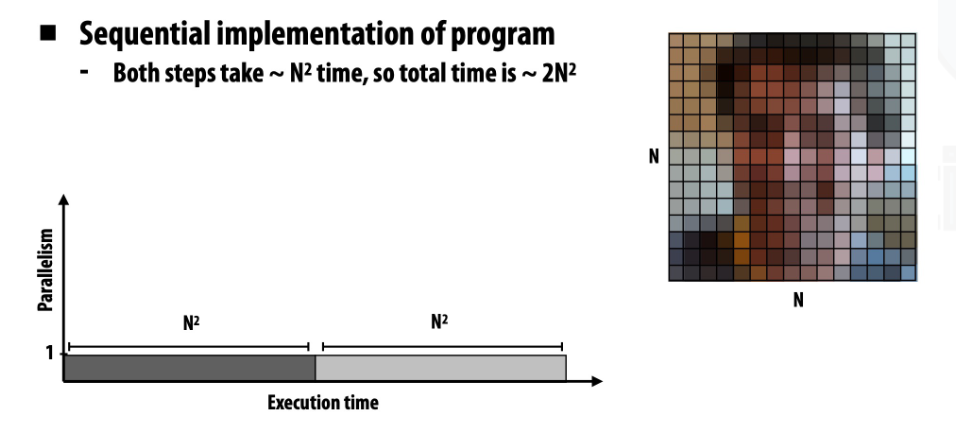
\includegraphics[width=0.7\linewidth]{img/esecuzione-sequenziale.png}
	\caption{Esecuzione sequenziale.}
	\label{fig:esecuzione-sequenziale}
\end{figure}

Una possibile strategia di parallelizzazione potrebbe consiste nell'eseguire in parallelo lo step 1, portando il tempo necessario a completare questa fase a $N^2/P$ (figure \ref{fig:esecuzione-parallela-1}), dove $P$ rappresenta il numero di processori disponibili. Lo speedup ottenuto sarebbe:
\begin{align*}
    speedup &\le \frac{2n^2}{\frac{n^2}{p} + n^2}\\
    &\le 2
\end{align*}

\begin{figure}[th]
	\centering
	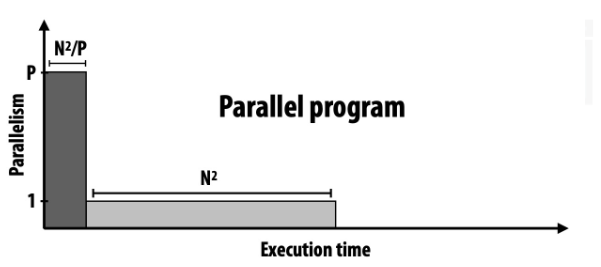
\includegraphics[width=0.7\linewidth]{img/esecuzione-parallela-1.png}
	\caption{Primo tentativo di parallelismo.}
	\label{fig:esecuzione-parallela-1}
\end{figure}

Una strategia più efficiente consiste nel parallelizzare parzialmente anche il secondo step, computando le somme parziali in parallelo (figure \ref{fig:esecuzione-parallela-2}). I tempi diventano:
\begin{align*}
    \text{Tempo step 1 } &= \frac{N^2}{P}\\
    \text{Tempo step 2 } &= \frac{N^2}{P} + P\\
\end{align*}

con speedup:
\begin{align*}
    speedup \le \frac{2n^2}{\frac{n^2}{p} + p}\\
\end{align*}

\begin{figure}[th]
	\centering
	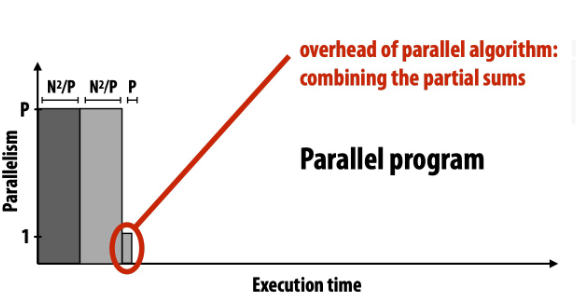
\includegraphics[width=0.7\linewidth]{img/esecuzione-parallela-2.png}
	\caption{Secondo tentativo di parallelismo.}
	\label{fig:esecuzione-parallela-2}
\end{figure}

\subsubsection{Assegnamento}
In questa fase andiamo a specificare il meccanismo con cui dividere le task tra i processi. Per semplicità, possiamo vedere le task come "cose da fare", mentre i processi/thread come i "lavoratori". Abbiamo fatto la scomposizione, sappiamo quanti e quali sono le thread, cerchiamo ora di fare un assegnamento che ci garantisca un certo livello di carico. 
Un approccio strutturato solitamente funziona bene, possiamo seguire euristiche ben conosciute o anche ispezionare attentamente il codice.


Il \textbf{load balancing} (bilanciamento del carico di lavoro) fa riferimento alla pratica di distribuzione delle task tra le thread affinchè tutte le thread siano occupate tutto il tempo. Possiamo anche definirlo come la riduzione al minimo dei tempi di inattività del processo. Questo passo è molto significativo per le perfromance. Ad esempio, se tutti i processi fossero soggetti ad un punto che funge da barriera di sincronizzazione, le performance globali verrebbero determinate dalla task più lenta.
\begin{figure}[th]
	\centering
	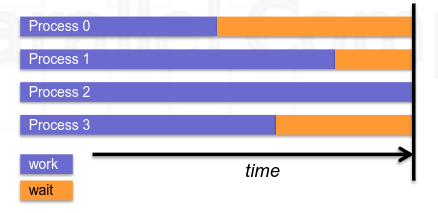
\includegraphics[width=0.7\linewidth]{img/barrier-sync.png}
	\caption{Esempi di punto di sincronizzazione.}
	\label{fig:barrier-sync}
\end{figure}

Possiamo ottenere il load balancing in più modi:
\begin{enumerate}
    \item Dividendo equamente le task tra i processi disponibili:
    \begin{itemize}
        \item In caso di operazioni su array/matrici, dove ogni processo esegue operazioni simili, il dataset viene distribuito in modo uniforme tra i processi;
        \item Per le iterazioni di un ciclo dove il lavoro svolto da ogni loop è similare, le iterazioni vengono distribuite uniformemente tra i processi;
        \item Se si utilizza un mix eterogeneo di macchine con performance variabili, è consigliato utilizzare dei tool di analisi delle performance per individuare carichi sbilanciati e aggiustare di conseguenza.
    \end{itemize}
    \item Usando un assegnamento dinamico del lavoro: alcune classi generano un carico di lavoro sbilanciato anche se i dati sono distribuiti egualmente tra il processi, come:
    \begin{itemize}
        \item Array sparsi;
        \item Adaptive grid methods, dove alcuni processi potrebbero dover perfezionare la propria mesh, mentre altri no;
        \item N-body simulations, dove alcune particelle potrebbero migrare verso/dal dominio del proprio processo di origine verso quello di un altro processo, oppure dove alcune particelle richiedono più lavoro rispetto ad altre.
    \end{itemize}
    Quando l'ammontare di lavoro che ogni thread performerà è variabile (non intenzionalmente ovviamente), è utile usare un approccio \textbf{scheduler – task pool}. In questo modo, appena un processo finisce, si mette in coda per ottenere un nuovo pezzo di lavoro.
    Inoltre, potrebbe diventare necessario disegnare un algoritmo che rileva e gestire sbilanciamento mentre questi si verificano dinamicamente nel codice.
\end{enumerate}

La \textbf{granularità} rappresenta una misura qualitativa del rapporto tra computazione e comunicazione. Generalmente i periodi di computazione sono separati da quelli di comunicazione da eventi di sincronizzazione. Relativamente al parallelismo, la granularità si divide in:
\begin{itemize}
    \item Fine grain parallelism (parallelismo a grana fine): si effettuano relativamente piccole quantità di lavoro computazionale tra gli eventi di comunicazione. Abbiamo quindi un basso rateo tra computazione e comunicazione. Facilita il load balancing; implica un elevato overhead di comunicazione e meno opportunità per il miglioramento delle performance. Se la granularità è troppo fine è possibile che l'overhead richiesto per comunicazione ee sincronizzazione tra le task richieda più tempo della computazione vera e propria.





    \item Coarse grain parallelism (parallelismo a grana grossa): si effettuano relativamente grandi quantità di lavoro computazionale tra gli eventi di comunicazione/sincronizzazione. Abbiamo quindi un alto rateo tra computazione e comunicazione. Implica più opportunità per un incremento delle performance, ma rende più difficile bilanciare il carico di lavoro efficientemente
\end{itemize}














\end{document}